\begin{figure}[t!]
\begin{tabular}{@{}c@{}c@{}c@{}}
\begin{subfigure}[b]{0.26\textwidth}
\begin{center}
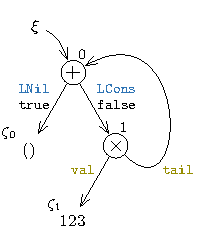
\includegraphics[scale=1.3]{chapters/figures/figValueTreeList2.pdf}
\end{center}
\vspace{24px}
\caption{\label{fig:valuetreelist1}\cons{LNil}}
\end{subfigure}%
&
\begin{subfigure}[b]{0.42\textwidth}
\begin{center}
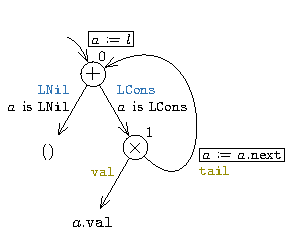
\includegraphics[scale=1.3]{chapters/figures/figValueTreeVarList.pdf}
\end{center}
\vspace{18px}
\caption{\label{fig:valuetreevarlist}$l\ctype{List}$}
\end{subfigure}%
&
\begin{subfigure}[b]{0.32\textwidth}
\begin{center}
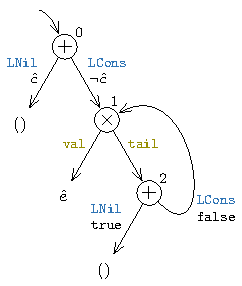
\includegraphics[scale=1.3]{chapters/figures/figValueTreeList1.pdf}
\end{center}
\caption{\label{fig:valuetreelist2}\sumIf{p=0} \sumThen{\cons{LNil}} \\ \qquad\  \sumElse{\cons{LCons}(42, \cons{LNil})}}
\end{subfigure}%
\\
\end{tabular}
\caption{\label{fig:valuetrees}Value trees of three \type{List}-typed expressions}
\end{figure}